\documentclass[nofonts,]{tufte-handout}

% ams
\usepackage{amssymb,amsmath}

\usepackage{ifxetex,ifluatex}
\usepackage{fixltx2e} % provides \textsubscript
\ifnum 0\ifxetex 1\fi\ifluatex 1\fi=0 % if pdftex
  \usepackage[T1]{fontenc}
  \usepackage[utf8]{inputenc}
\else % if luatex or xelatex
  \makeatletter
  \@ifpackageloaded{fontspec}{}{\usepackage{fontspec}}
  \makeatother
  \defaultfontfeatures{Ligatures=TeX,Scale=MatchLowercase}
  \makeatletter
  \@ifpackageloaded{soul}{
     \renewcommand\allcapsspacing[1]{{\addfontfeature{LetterSpace=15}#1}}
     \renewcommand\smallcapsspacing[1]{{\addfontfeature{LetterSpace=10}#1}}
   }{}
  \makeatother
\fi

% graphix
\usepackage{graphicx}
\setkeys{Gin}{width=\linewidth,totalheight=\textheight,keepaspectratio}

% booktabs
\usepackage{booktabs}

% url
\usepackage{url}

% hyperref
\usepackage{hyperref}

% units.
\usepackage{units}


\setcounter{secnumdepth}{-1}

% citations
\usepackage{natbib}
\bibliographystyle{plainnat}

%% tint override
\setcitestyle{round} 

% pandoc syntax highlighting

% longtable
\usepackage{longtable,booktabs}

% multiplecol
\usepackage{multicol}

% strikeout
\usepackage[normalem]{ulem}

% morefloats
\usepackage{morefloats}


% tightlist macro required by pandoc >= 1.14
\providecommand{\tightlist}{%
  \setlength{\itemsep}{0pt}\setlength{\parskip}{0pt}}

% title / author / date
\title{Genetic engineering and gene cloning}
\author{Deependra Dhakal}
\date{2019-06-15}

%% -- tint overrides
%% fonts, using roboto (condensed) as default
\usepackage[sfdefault,condensed]{roboto}
%% also nice: \usepackage[default]{lato}

%% colored links, setting 'borrowed' from RJournal.sty with 'Thanks, Achim!'
\RequirePackage{color}
\definecolor{link}{rgb}{0.1,0.1,0.8} %% blue with some grey
\hypersetup{
  colorlinks,%
  citecolor=link,%
  filecolor=link,%
  linkcolor=link,%
  urlcolor=link
}

%% macros
\makeatletter

%% -- tint does not use italics or allcaps in title
\renewcommand{\maketitle}{%     
  \newpage
  \global\@topnum\z@% prevent floats from being placed at the top of the page
  \begingroup
    \setlength{\parindent}{0pt}%
    \setlength{\parskip}{4pt}%
    \let\@@title\@empty
    \let\@@author\@empty
    \let\@@date\@empty
    \ifthenelse{\boolean{@tufte@sfsidenotes}}{%
      %\gdef\@@title{\sffamily\LARGE\allcaps{\@title}\par}%
      %\gdef\@@author{\sffamily\Large\allcaps{\@author}\par}%
      %\gdef\@@date{\sffamily\Large\allcaps{\@date}\par}%
      \gdef\@@title{\begingroup\fontseries{b}\selectfont\LARGE{\@title}\par}%
      \gdef\@@author{\begingroup\fontseries{l}\selectfont\Large{\@author}\par}%
      \gdef\@@date{\begingroup\fontseries{l}\selectfont\Large{\@date}\par}%
    }{%
      %\gdef\@@title{\LARGE\itshape\@title\par}%
      %\gdef\@@author{\Large\itshape\@author\par}%
      %\gdef\@@date{\Large\itshape\@date\par}%
      \gdef\@@title{\begingroup\fontseries{b}\selectfont\LARGE\@title\par\endgroup}%
      \gdef\@@author{\begingroup\fontseries{l}\selectfont\Large\@author\par\endgroup}%
      \gdef\@@date{\begingroup\fontseries{l}\selectfont\Large\@date\par\endgroup}%
    }%
    \@@title
    \@@author
    \@@date
  \endgroup
  \thispagestyle{plain}% suppress the running head
  \tuftebreak% add some space before the text begins
  \@afterindentfalse\@afterheading% suppress indentation of the next paragraph
}

%% -- tint does not use italics or allcaps in section/subsection/paragraph
\titleformat{\section}%
  [hang]% shape
  %{\normalfont\Large\itshape}% format applied to label+text
  {\fontseries{b}\selectfont\Large}% format applied to label+text
  {\thesection}% label
  {1em}% horizontal separation between label and title body
  {}% before the title body
  []% after the title body

\titleformat{\subsection}%
  [hang]% shape
  %{\normalfont\large\itshape}% format applied to label+text
  {\fontseries{m}\selectfont\large}% format applied to label+text
  {\thesubsection}% label
  {1em}% horizontal separation between label and title body
  {}% before the title body
  []% after the title body

\titleformat{\paragraph}%
  [runin]% shape
  %{\normalfont\itshape}% format applied to label+text
  {\fontseries{l}\selectfont}% format applied to label+text
  {\theparagraph}% label
  {1em}% horizontal separation between label and title body
  {}% before the title body
  []% after the title body

%% -- tint does not use italics here either
% Formatting for main TOC (printed in front matter)
% {section} [left] {above} {before w/label} {before w/o label} {filler + page} [after]
\ifthenelse{\boolean{@tufte@toc}}{%
  \titlecontents{part}% FIXME
    [0em] % distance from left margin
    %{\vspace{1.5\baselineskip}\begin{fullwidth}\LARGE\rmfamily\itshape} % above (global formatting of entry)
    {\vspace{1.5\baselineskip}\begin{fullwidth}\fontseries{m}\selectfont\LARGE} % above (global formatting of entry)
    {\contentslabel{2em}} % before w/label (label = ``II'')
    {} % before w/o label
    {\rmfamily\upshape\qquad\thecontentspage} % filler + page (leaders and page num)
    [\end{fullwidth}] % after
  \titlecontents{chapter}%
    [0em] % distance from left margin
    %{\vspace{1.5\baselineskip}\begin{fullwidth}\LARGE\rmfamily\itshape} % above (global formatting of entry)
    {\vspace{1.5\baselineskip}\begin{fullwidth}\fontseries{m}\selectfont\LARGE} % above (global formatting of entry)
    {\hspace*{0em}\contentslabel{2em}} % before w/label (label = ``2'')
    {\hspace*{0em}} % before w/o label
    %{\rmfamily\upshape\qquad\thecontentspage} % filler + page (leaders and page num)
    {\upshape\qquad\thecontentspage} % filler + page (leaders and page num)
    [\end{fullwidth}] % after
  \titlecontents{section}% FIXME
    [0em] % distance from left margin
    %{\vspace{0\baselineskip}\begin{fullwidth}\Large\rmfamily\itshape} % above (global formatting of entry)
    {\vspace{0\baselineskip}\begin{fullwidth}\fontseries{m}\selectfont\Large} % above (global formatting of entry)
    {\hspace*{2em}\contentslabel{2em}} % before w/label (label = ``2.6'')
    {\hspace*{2em}} % before w/o label
    %{\rmfamily\upshape\qquad\thecontentspage} % filler + page (leaders and page num)
    {\upshape\qquad\thecontentspage} % filler + page (leaders and page num)
    [\end{fullwidth}] % after
  \titlecontents{subsection}% FIXME
    [0em] % distance from left margin
    %{\vspace{0\baselineskip}\begin{fullwidth}\large\rmfamily\itshape} % above (global formatting of entry)
    {\vspace{0\baselineskip}\begin{fullwidth}\fontseries{m}\selectfont\large} % above (global formatting of entry)
    {\hspace*{4em}\contentslabel{4em}} % before w/label (label = ``2.6.1'')
    {\hspace*{4em}} % before w/o label
    %{\rmfamily\upshape\qquad\thecontentspage} % filler + page (leaders and page num)
    {\upshape\qquad\thecontentspage} % filler + page (leaders and page num)
    [\end{fullwidth}] % after
  \titlecontents{paragraph}% FIXME
    [0em] % distance from left margin
    %{\vspace{0\baselineskip}\begin{fullwidth}\normalsize\rmfamily\itshape} % above (global formatting of entry)
    {\vspace{0\baselineskip}\begin{fullwidth}\fontseries{m}\selectfont\normalsize\rmfamily} % above (global formatting of entry)
    {\hspace*{6em}\contentslabel{2em}} % before w/label (label = ``2.6.0.0.1'')
    {\hspace*{6em}} % before w/o label
    %{\rmfamily\upshape\qquad\thecontentspage} % filler + page (leaders and page num)
    {\upshape\qquad\thecontentspage} % filler + page (leaders and page num)
    [\end{fullwidth}] % after
}{}

  
\makeatother


\usepackage{booktabs}
\usepackage{longtable}
\usepackage{array}
\usepackage{multirow}
\usepackage{wrapfig}
\usepackage{float}
\usepackage{colortbl}
\usepackage{pdflscape}
\usepackage{tabu}
\usepackage{threeparttable}
\usepackage{threeparttablex}
\usepackage[normalem]{ulem}
\usepackage{makecell}
\usepackage{xcolor}

\begin{document}

\maketitle




\clearpage

\hypertarget{genetic-engineering}{%
\section{Genetic engineering}\label{genetic-engineering}}

\hypertarget{genetic-engineering-in-plants}{%
\subsection{Genetic engineering in
plants}\label{genetic-engineering-in-plants}}

In general, plants are genetically engineered to increase yield or to
confer resistance to drought or pests. Finding desirable genes can be
difficult because multiple interacting genes usually control such
traits. In addition, such genes may play other roles in plant physiology
or development. So far, most successful genetic engineering of plants
has relied on inserting one or a few genes that supply simple, yet
useful, properties.

For example, resistance to the herbicide glyphosate is due to a single
gene. Making a crop such as soybeans resistant to glyphosate allows the
farmer to kill the weeds in the field without harming the soybeans.
Another desirable trait often due to a single gene is the production of
toxins that kill harmful insects. Also, a two-gene pathway has been
engineered into rice to make it more resistant to drought. Before
discussing these examples, however, we must first describe how
transgenic plants are created.

\hypertarget{ti-plasmid}{%
\subsection{Ti Plasmid}\label{ti-plasmid}}

Plants suffer from tumors although they are quite different from the
cancers of animals. The most common cause is the \emph{Ti plasmid}
(tumor-inducing plasmid), which is carried by soil bacteria of the
\emph{Agrobacterium} group. The most important aspect of the infection
is that a specific segment of the Ti plasmid DNA is transferred from the
bacteria to the plant. Because most DNA transfers occur only between
closely related organisms, the ability of \emph{Agrobacterium} to
transfer DNA from one domain to another makes it an important tool for
the genetic engineering of plants.

\begin{figure}
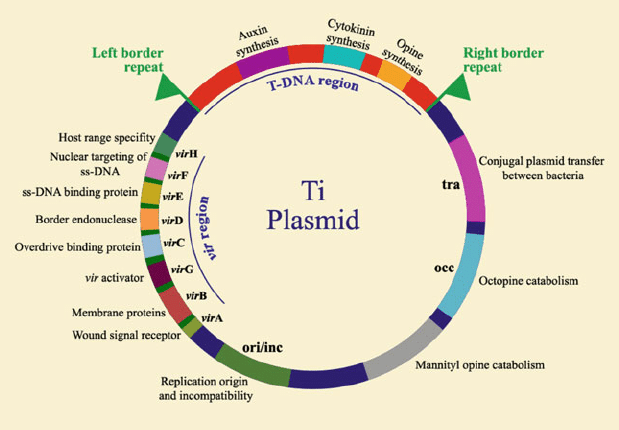
\includegraphics[width=0.9\linewidth]{./images/Ti_plasmid} \caption[The structure of the Ti plasmid]{The structure of the Ti plasmid}\label{fig:ti-plasmid}
\end{figure}

In nature, \emph{Agrobacterium} is attracted to plants that have minor
wounds by phenolic compounds such as acetosyringone, which are released
at the wound. These chemicals induce the bacteria to move and attach to
the plant via a variety of cell surface receptors. The same inducers
activate expression of the virulence genes on the Ti plasmid that are
responsible for DNA transfer to the plant. This is under control of a
two-component regulatory system.

\begin{marginfigure}
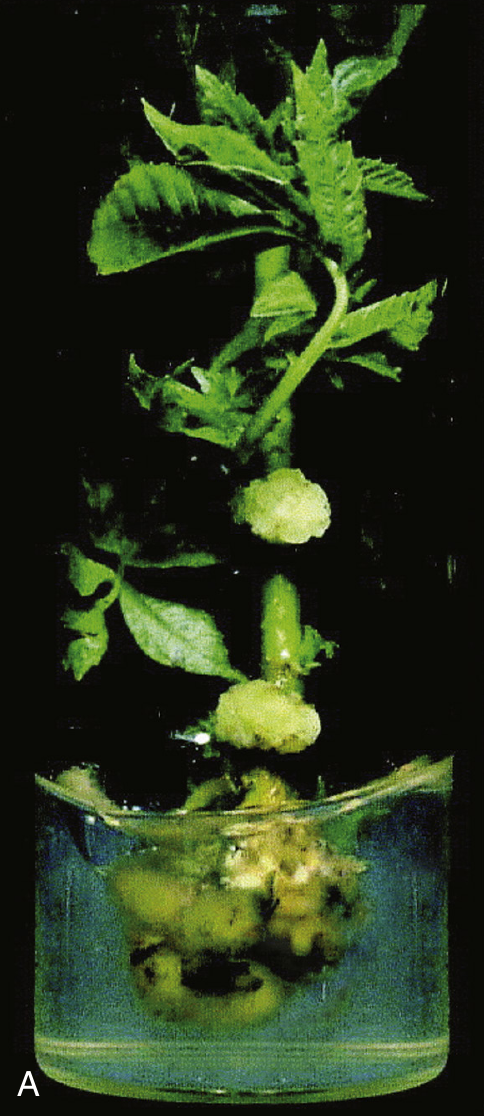
\includegraphics[width=0.7\linewidth]{./images/agrobacterium_gall_a} \caption[Crown gall tumors are caused by Agrobacterium tumefaciens]{Crown gall tumors are caused by Agrobacterium tumefaciens}\label{fig:agrobacterium-gall}
\end{marginfigure}
\begin{marginfigure}
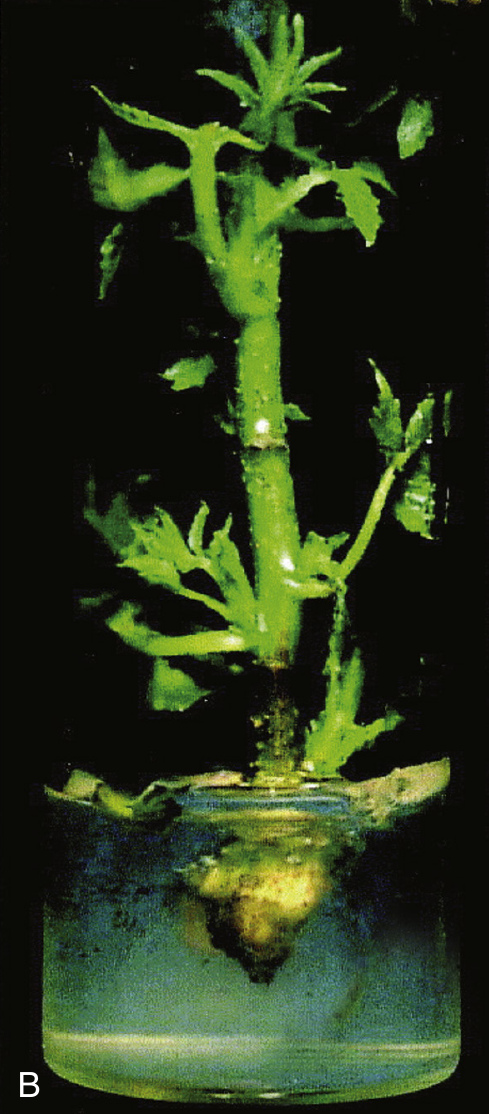
\includegraphics[width=0.7\linewidth]{./images/agrobacterium_gall_b} \caption[But plants expressing inhibitors of key proteins for Agrobacterium infection do not develop any tumors (B)\newline Crown gall disease in walnut (Juglans regia L.)]{But plants expressing inhibitors of key proteins for Agrobacterium infection do not develop any tumors (B)\newline Crown gall disease in walnut (Juglans regia L.)}\label{fig:agrobacterium-gall}
\end{marginfigure}

At the cell surface, the sensor, VirA, is autophosphorylated when it
detects the plant phenolic compounds. Next, VirA transfers the phosphate
to the DNA-binding protein, VirG, which activates transcription of the
vir genes of the Ti plasmid. Two of the gene products (VirD1 and VirD2)
clip the T-DNA borders to form a single-stranded immature T-complex.
VirD2 then attaches to the \(5^\prime\) end of the T-DNA, and bacterial
helicases unwind the T-DNA from the plasmid. The single-stranded gap on
the plasmid is repaired, and the T-DNA is coated with VirE2 protein to
give a hollow cylindrical filament with a coiled structure. This is the
mature form of T-DNA and traverses into the plant.

The Ti plasmid is lost when Agrobacterium is grown above \(28^\circ C\).
Such cured bacteria do not induce crown galls, i.e.~they become
avirulent. pTi and pRi share little sequence homology but are
functionally rather similar. The Ti plasmids are classified into
different types based on the type of opine produced by their genes. The
different opines specified by pTi are octopine, nopaline, succinamopine
and leucinopine.

The plasmid has 196 genes that code for 195 proteins. There is one
structural RNA. The plasmid is 206,479 nucleotides long, the GC content
is 56\% and 81\% of the material is coding genes. There are no
pseudogenes.

\emph{Virulence region}

Genes in the virulence region are grouped into the operons virABCDEFG,
which code for the enzymes responsible for mediating conjugative
transfer of T-DNA to plant cells \citep{stachel1986genetic}.

\begin{itemize}
\tightlist
\item
  virA codes for a receptor which reacts to the presence of phenolic
  compounds such as acetosyringone, syringealdehyde or acetovanillone
  which leak out of damaged plant tissues.
\item
  virB encodes proteins which produce a pore/pilus-like structure.
\item
  virC binds the overdrive sequence.
\item
  virD1 and virD2 produce endonucleases which target the direct repeat
  borders of the T-DNA segment; virD4 is the coupling protein.
\item
  virE binds to T-strand protecting it from nuclease attack, and
  intercalates with lipids to form channels in the plant membranes
  through which the T-complex passes, beginning with the right border.
\item
  virG activates vir-gene expression after binding to a consensus
  sequence, once it has been phosphorylated by virA.
\end{itemize}

T-DNA transfer to the plant is similar to bacterial conjugation. First,
Agrobacterium forms a pilus. This rod-like structure forms a connection
with the plant cell and opens a channel through which the T-DNA is
actively transported into the plant cytoplasm. Both pilus and transport
complex consist of proteins that are vir gene products. Once inside the
plant cytoplasm, T-DNA is imported into the nucleus. Both VirE2 and
VirD2 have nuclear localization signals that are recognized by plant
cytosolic proteins. These proteins take the T-complex to the nucleus,
where it is actively transported through a nuclear pore. The single
T-DNA strand is integrated directly into the plant genome and converted
to a double-stranded form. The integration requires DNA ligase,
polymerase, and chromatin remodeling proteins, all of which are supplied
by the plant.

Once integrated, the genes in the T-DNA are expressed. These genes have
eukaryote-like promoters, transcriptional enhancers, and poly(A) sites
and therefore are expressed in the plant nucleus rather than in the
original bacterium. The proteins they encode synthesize two plant
hormones: auxin and cytokinin. Auxin makes plant cells grow bigger, and
cytokinin makes them divide. The infected plant cells begin to grow
rapidly and without control, resulting in a tumor (Figure
\ref{fig:agrobacterium-gall}). T-DNA also carries genes for the
synthesis of a variety of different amino acid and sugar phosphate
derivatives called opines. Strains of Agrobacterium are differentiated
based on the kinds of opines they produce. Opines are made by plant
cells that contain T-DNA, but they cannot be utilized by the plant. The
Ti plasmid, which is still inside the Agrobacterium, carries genes that
allow the bacteria to utilize them. Thus, the bacterium has hijacked the
plant's metabolic machinery into supplying the bacteria with food. Other
bacteria, which might be present by chance, cannot use opines because
they do not possess the genes for their uptake and metabolism.

Molecular biologists have commandeered Ti plasmids to genetically
engineer plants. The Ti plasmid has been disarmed by removing the genes
for plant hormone and opine synthesis from the T-DNA and streamlined the
plasmid by removing genes that are not involved in transferring the
T-DNA. (These smaller plasmids are much easier to work with and can be
manipulated in Escherichia coli rather than their original host,
Agrobacterium.) A transgene of interest, such as an insect toxin gene,
is inserted into the T-DNA region of the Ti plasmid. When the T-DNA
enters the plant cell and integrates into the chromosome, it will bring
in the transgene instead of causing a tumor.

The transferred region of the plasmid must also have other elements in
order for this technique to be successful (Figure \ref{fig:ti-plasmid}).
The genetically modified T-DNA region must contain a selectable marker,
such as an herbicide or antibiotic resistance gene that is used to track
whether the foreign DNA has been inserted into plant cells. Expression
of the transgene requires a promoter that works efficiently in plant
cells. It may be one of two types. A constitutive promoter will turn the
gene on in all the plant cells throughout development; thus, every
tissue, even the fruit or seed, will express the gene. A more refined
approach is to use an inducible promoter that acts as an on/off switch.
An example of this is the cab promoter from the gene encoding
chlorophyll a/b binding protein. This promoter is turned on only when
the plant is exposed to light; therefore, root tissues and tubers such
as potatoes will not express the gene. Many different promoters may be
used, but ideally, the promoter should turn on only in tissues that need
transgene function.

\begin{figure*}
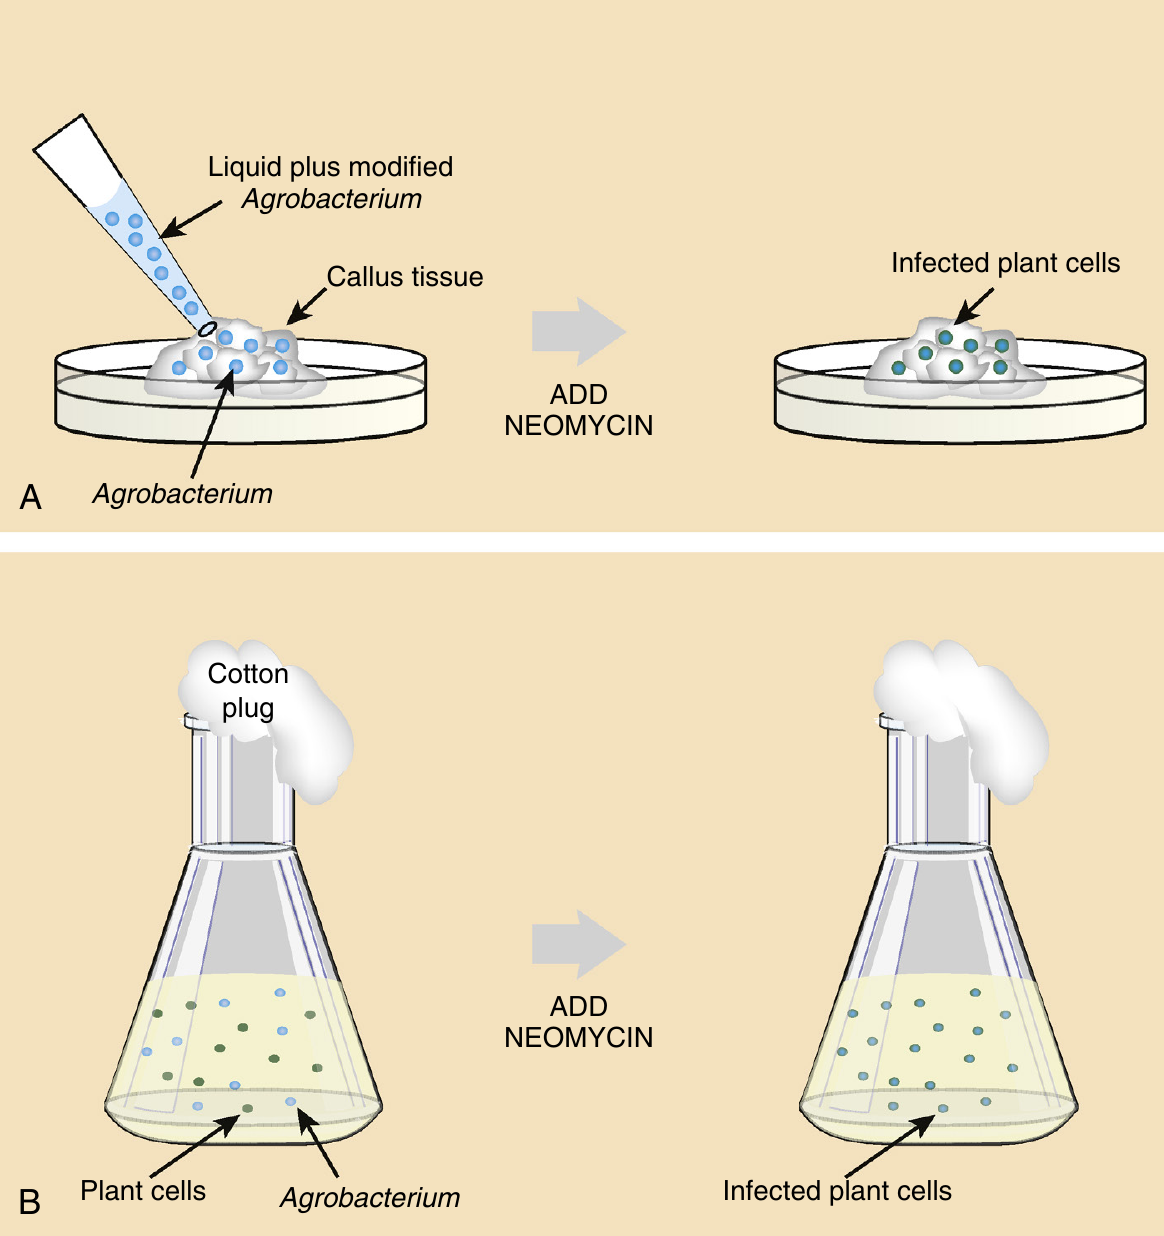
\includegraphics[width=0.95\linewidth]{./images/agrobacterium_infection_culture} \caption{\textbf{Transfer of modified Ti plasmid into a plant.} Agrobacterium carrying a Ti plasmid is added to plant tissue growing in culture. The T-DNA carries an antibiotic resistance gene (neomycin in this figure) to allow selection of successfully transformed plant cells. Both callus cultures (A) and liquid cultures (B) may be used in this procedure.}\label{fig:agrobacterium-infection-culture}
\end{figure*}

In practice, Agrobacterium is used to transfer genes of interest into
plants using tissue culture. Either protoplasts or a piece of callus are
cultured with Agrobacterium harboring a Ti plasmid with modified T-DNA.
After coculture, the plant cells are harvested and incubated with the
herbicide or antibiotic used as the selectable marker. This kills all
the cells that were not transformed with T-DNA or failed to express the
genes on the T-DNA (Figure \ref{fig:agrobacterium-infection-culture}).
The transformed plant cells are then induced to produce shoot and root
tissue by altering the hormone conditions in the medium. The small
transgenic plants can then be screened for transgene expression levels.

\begin{figure*}
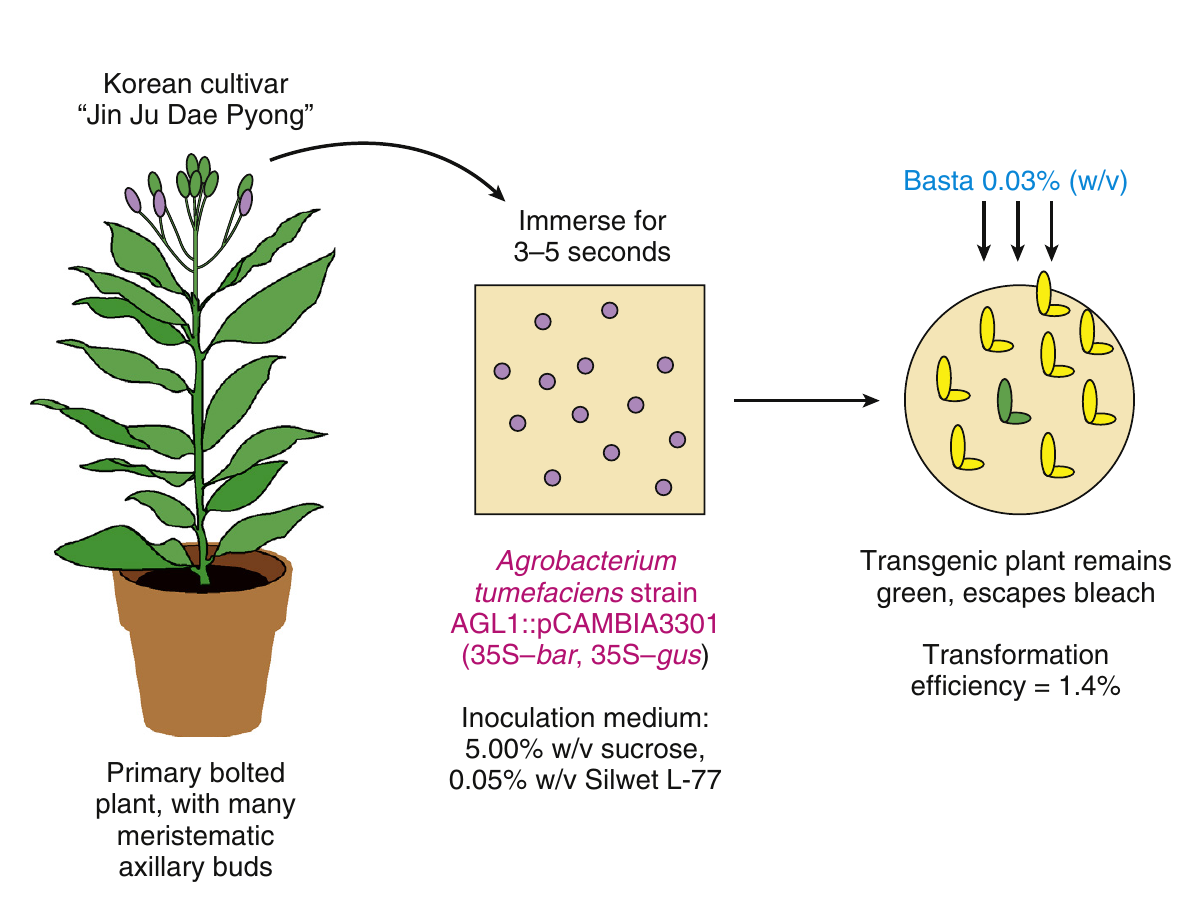
\includegraphics[width=0.95\linewidth]{./images/agrobacterium_infection_intact} \caption[\textbf{Floral dip method of plant transformation} Flower buds exposed to Agrobacterium containing modified T-DNA can result in the production of transgenic seeds]{\textbf{Floral dip method of plant transformation} Flower buds exposed to Agrobacterium containing modified T-DNA can result in the production of transgenic seeds. Adapted from Curtis IS (2003). The noble radish: past, present and future. Trends Plant Sci 8, 305–307.}\label{fig:agrobacterium-infection-intact}
\end{figure*}

Recently, a method for in planta Agrobacterium transformation was
developed and has revolutionized plant transgenics. In planta
transformation is also known as the floral dip method (Figure
\ref{fig:agrobacterium-infection-intact}). The method was developed
using the model plant Arabidopsis but has been extended to other plants,
such as wheat and maize. First, Arabidopsis plants are grown until
flower buds begin to form. These buds are removed and allowed to
regenerate for a few days. Once they begin to regenerate, the plants are
dipped into a suspension of Agrobacterium containing a surfactant, which
decreases surface tension and allows the Agrobacterium to adhere to the
plant and transfer its T-DNA. Because the flower buds are just beginning
to form, the T-DNA becomes part of the germline through the ovarian
tissue. The plant is allowed to finish growing and produce seed. These
seeds are harvested and grown in selective media to find those that have
integrated and expressed T-DNA. Although the method gives a low
percentage of transformants, so many seeds can be screened that the
overall procedure works well.

\hypertarget{particle-bombardment}{%
\subsection{Particle Bombardment}\label{particle-bombardment}}

Another strategy for getting a transgene into plant tissue is particle
bombardment (Figure \ref{fig:gene-gun-transfer}). A gun blasts
microscopic metal particles carrying DNA through the tough plant cell
walls. Unlike Ti plasmid transfer by Agrobacterium, this technique works
with all types of plants. Though the technique is nonspecific, it has
been very successful.

First, either a leaf disk (a round piece of leaf tissue) or a callus is
isolated from the plant, placed on a dish, and put in a vacuum chamber.
The DNA to be inserted (carrying the transgene, proper regulatory
elements, and selectable marker) is coated on microscopic gold beads.
The beads are placed at the end of chamber. One variant of the method
uses a blast of air or helium to drive the filter containing the gold
beads toward the stop screen and sample. In the first gene guns, actual
firearm blanks were used to accelerate the bullet. Between the bullet
and plant tissue is a stop plate. Filter and gold beads hit this stop
screen, the DNA-coated beads are thrown forward into the plant tissue.
An alternative method is to accelerate the beads by a strong electrical
discharge. The high voltage vaporizes a water droplet, and the resulting
shock wave proels a thin metal sheet covered with the particles at a
mesh screen. The screen blocks the metal sheet but allows the DNA-coated
particles to accelerate through into the plant tissue. One advantage of
this method is that the strength of the electrical discharge can be
controlled; therefore, the amount of penetration into the tissue can be
regulated.

\begin{figure}
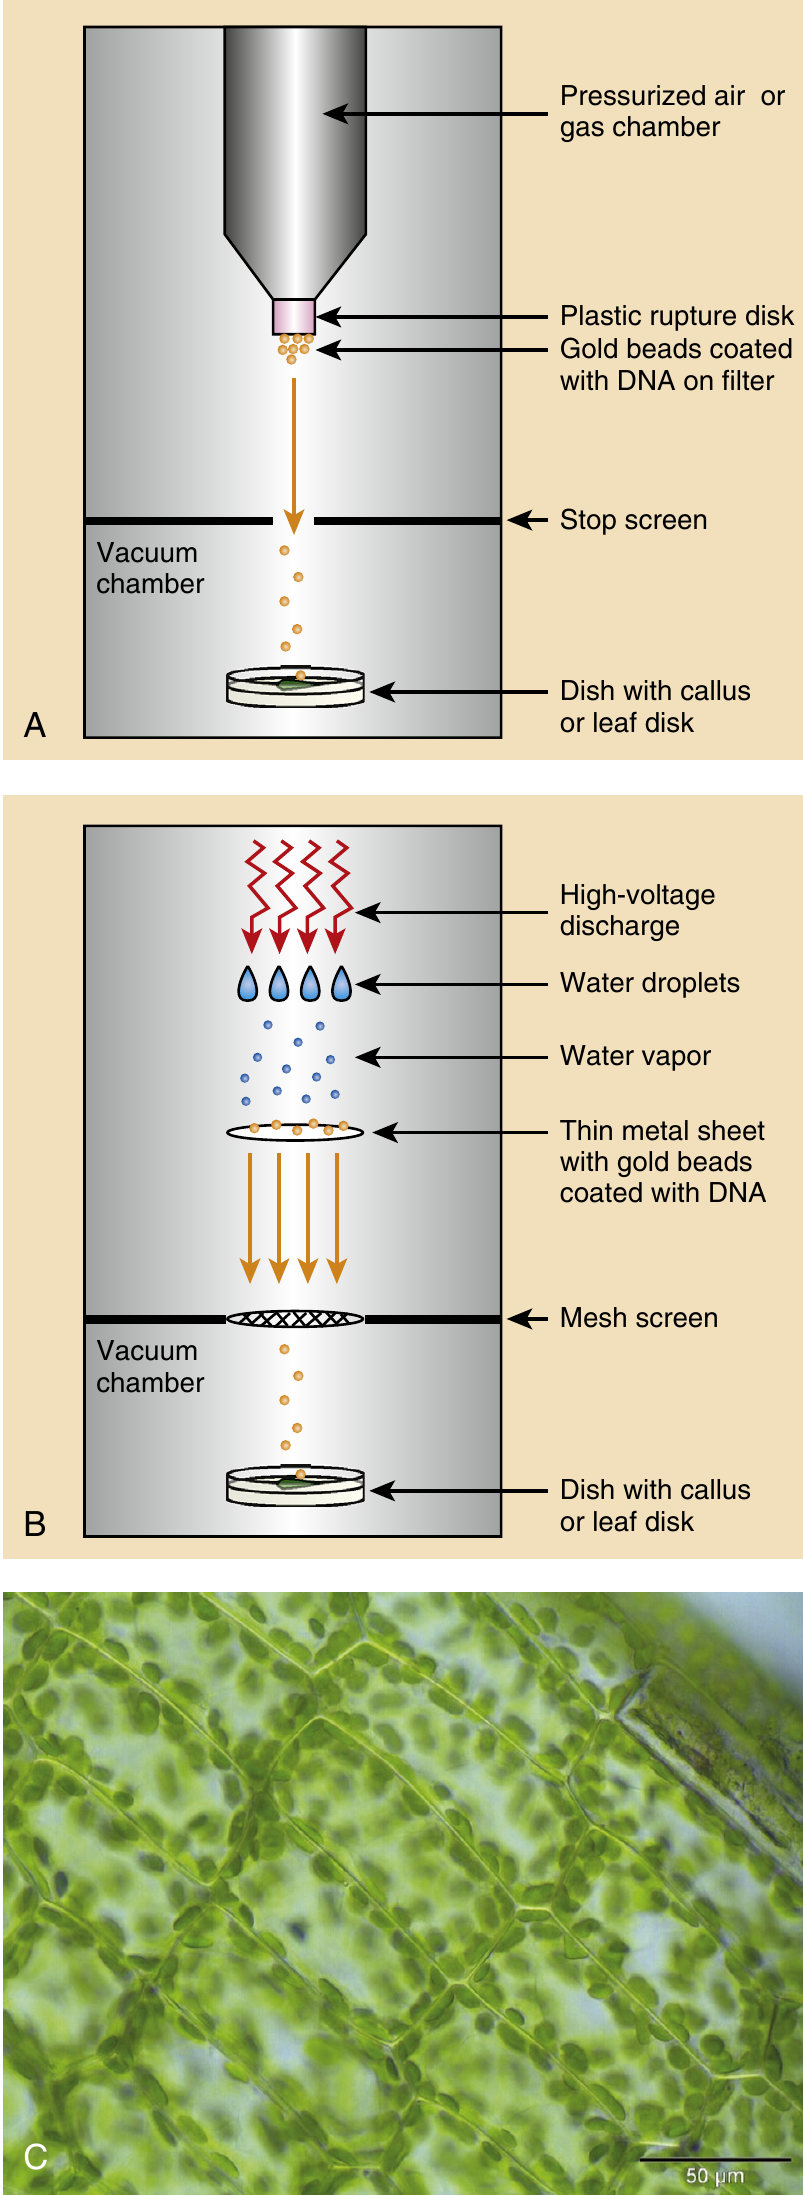
\includegraphics[width=0.9\linewidth]{./images/gene_gun_transfer} \caption[A gene gun that operates via (A) pressurized air or (B) high-voltage discharge is depicted]{A gene gun that operates via (A) pressurized air or (B) high-voltage discharge is depicted. In both cases, the stop plate halts the projectile, and the microscopic metal particles carrying the DNA penetrate the plant tissue.}\label{fig:gene-gun-transfer}
\end{figure}

\hypertarget{detecting-the-inserted-dna}{%
\subsection{Detecting the inserted
DNA}\label{detecting-the-inserted-dna}}

Simplest of all ways to detect the inserted DNA is to include a
selectable marker or reporter gene on the same segment of DNA as the
transgene. One widely used reporter gene is \emph{npt}, which encodes
neomycin phosphotransferase. This enzyme confers neomycin resistance by
attaching a phosphate group to the molecule. Transformed cells are
directly selected with the antibiotic neomycin, which kills any cells
that did not integrate the DNA.

An alternative reporter gene encodes for luciferase. This enzyme emits
light when provided with its substrate, luciferin. Although high-level
expression of luciferase can be seen with the naked eye, usually the
amount of light is small and must be detected with sensitive electronic
apparatus such as scintillation counter, a photocell detector, or a
charge-coupled device camera. This reporter gene has a key advantage in
that the luciferase protein is not stable for long time, so the amount
of active protein correlates with the level of gene expression at any
given time. Therefore, \emph{luc} can be used to determine the activity
of specific promoters.

Removal of selectable markers (genes), which may even have unfounded
concerns in the public is catalyzed by \emph{Cre/lox} P gene system,
which produces Cre (``Causes recombination'') protein, that recognized
34 base-pair DNA sequence, the \emph{\emph{loxP}} site. The Cre protein
catalyzes recombination between two loxP sites.

\begin{figure}
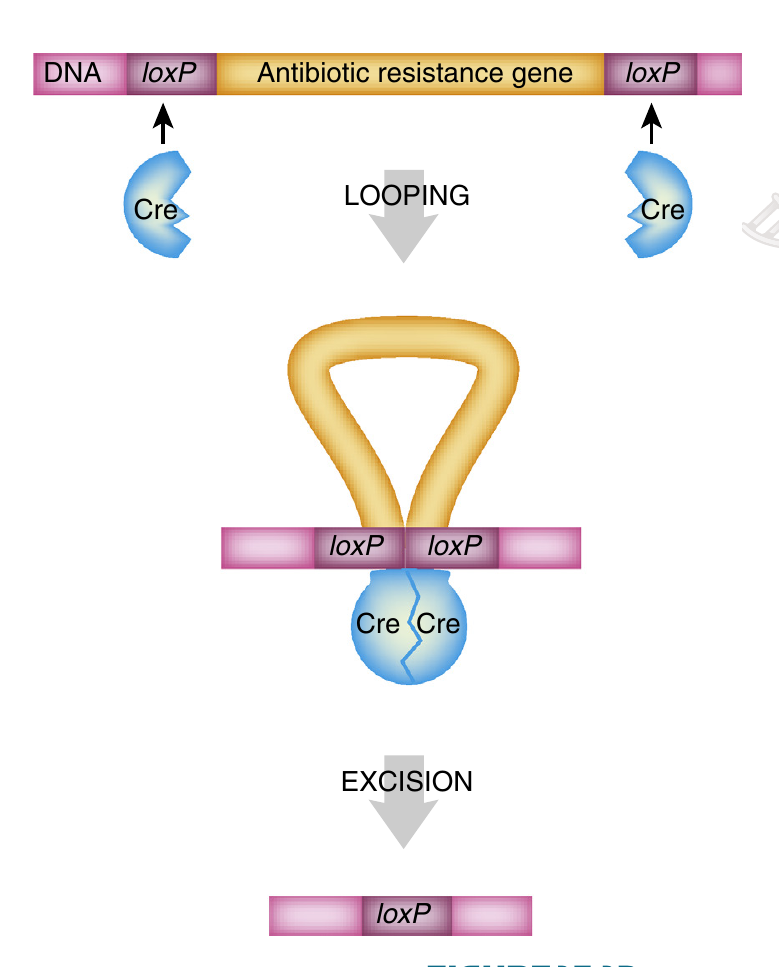
\includegraphics[width=0.9\linewidth]{./images/marker_removal} \caption{\textbf{The Cre/\textit{lox}P System of Bacteriophage P1}\newline The Cre protein binds to \textit{lox}P recognition sites in the DNA. Two nearly \textit{lox}P sites are brought together, and recombination between them eliminates the intervening DNA. A single \textit{lox}P 'scar' site remains in the target DNA molecule}\label{fig:marker-removal}
\end{figure}

The cre gene can be added to the system by cross-pollination of two
different plants: One plant carrying the transgene plus a selectable
marker that is flanked by two \emph{lox} P sites is crossed with another
plant carrying the \emph{cre} gene. First, the \emph{lox} P pollen from
the plant with the \emph{cre} gene is added to the stigma of the plant
with the transgene. The resulting seeds are grown and checked for
sensitivity to the selective agent (e.g., neomycin). If the Cre protein
is present in the progeny, the selectable marker gene will be excised
and lost during growth. This plant now has the transgene and the cre
gene, but no longer has the gene for antibiotic resistance.

\hypertarget{genetically-engineered-crops}{%
\subsection{Genetically engineered
crops}\label{genetically-engineered-crops}}

A task force of the Codex Alimentarius Commission, a U.N. agency
responsible for an international code for food standardization, has
advanced the following language to standardize the labeling of foods
derived from GMOs for purposes of international commerce:

\begin{quote}
``Genetically modified/engineered organism means an organism in which
the genetic material has been changed through gene technology in a way
that does not occur naturally by multiplication and/or any natural
recombination.''
\end{quote}

Corn lines have been modified to express:

\begin{itemize}
\tightlist
\item
  tolerance to either the herbicide glyphosate (RoundUp(R)), or to the
  herbicide glufosinate-ammonium (Liberty(R));
\item
  resistance to the pest, european corn borer (Ostrinia nubilalis) ECB;
\item
  or a combination of herbicide tolerance to either glyphosate or
  glufosinate-ammonium and ECB resistance.
\end{itemize}

Soybean lines have been modified to express:

\begin{itemize}
\tightlist
\item
  tolerance to either glyphosate, or to (Liberty),
\item
  modified oil (high oleic acid) content.
\end{itemize}

Cotton lines have been modified to express:

\begin{itemize}
\tightlist
\item
  herbicide tolerance to either glyphosate, bromoxynil or sulfonylurea,
\item
  insect resistance to the pest, pink bollworm (Pectinophora
  gossypiella) PBW and tobacco budworm (Heliothis virescens) TBW.
\item
  bromoxynil tolerance and PBW resistance.
\end{itemize}

Tomato lines have been modified to:

\begin{itemize}
\tightlist
\item
  delay fruit ripening
\item
  express resistance to the pests tomato pinworm, (Kieferia
  lycopersicella) TPW and tomato fruitworm (Helicoverpa zea) TFW
\item
  express a lower polygalacturonase level which makes for a more meaty
  tomato for processing.
\end{itemize}

Modified potato lines are:

\begin{itemize}
\tightlist
\item
  resistant to the Colorado Potato Beetle (Leptinotarsa decemlineata)
  CPB ,
\item
  expresses resistance to the potato virus Y (PVY) in addition to being
  resistant to the CPB.
\end{itemize}

Chapters:

\begin{itemize}
\item
  Genetically modified crop approvals and plant acerages

  \begin{itemize}
  \tightlist
  \item
    Molecular information and approval status of selected events
  \end{itemize}
\item
  Insect resistant transgenic crops
\item
  Transgenic technologies for insect resistance current achievements and
  future prospects
\item
  Genetic engineering of crops for improved weed management traits.
\end{itemize}

\hypertarget{references}{%
\section{References}\label{references}}

\begin{itemize}
\tightlist
\item
  Crop Biotechnology, American Chemical Society, 2002
\item
  Biotechnology, 2nd Edition, David P. Clark, Nanette J. Pazdernik
\end{itemize}

\bibliography{bibliographies.bib}



\end{document}
